Cassandra\cite{will10}, that was created on Facebook, first started as an incubation project at Apache in January of 2009 and is based on Dynamo \cite{Hastorun2007} and BigTable \cite{Chang2008}. This system can be defined as an open source, distributed, decentralized, elastically scalable, highly available, fault-tolerant, tuneably consistent, column-oriented database\cite{hewitt2010cassandra}. 

Cassandra is distributed, which means that it is capable of running on multiple machines while the users see it as if it was running in only one. More than that, Cassandra is built and optimized to run in more than one machine. So much that you cannot take full advantage of all of its features without doing so. In Cassandra, all of the nodes are identical, there is no such thing as a node that is responsible for certain organizing operations, as in BigTable or HBase. Instead, Cassandra features a peer-to-peer protocol and uses gossip to maintain and keep in sync a list of nodes that are alive or dead. 

Being decentralized means that there is no single point of failure, because all the servers are symmetrical. The main advantages of decentralization are that it is easier to use than master/slave and it helps to avoid suspension in service, thus supporting high availability.

Scalability is the ability to have little degradation in performance when facing a greater number of requests. It can be of two types:

\begin{description}
	\item[Vertical] Adding hardware capacity and/or memory
	\item[Horizontal] Adding more machines with all or some of the data so that all of it is replicated at least in two machines. The software must keep all the machines in sync. 
\end{description}

Elastic scalability refers to the capability of a cluster to seamlessly accept new nodes or removing them without any need to change the queries, rebalance data manually or restart the system.

Cassandra is highly available in the sense that if a node fails it can be replaced with no downtime and the data can be replicated through data centers to prevent that same downtime in the case of one of them experiencing a catastrophe, such as an earthquake or flood. 

Eric Brewer's CAP theorem \cite{Brewer2000} states that it is impossible for a distributed computer system to simultaneously provide all three of the following guarantees:
\begin{description}
	\item[Consistency] All clients see current data regardless of updates or deletes
	\item[Availability] All clients will always be able to read and write data, even with node failures
	\item[Partition Tolerance] The system continues to work as expected despite network or message failures
\end{description}

Figure \ref{fig:cap} provides a visual explanation of the theorem, with a focus on the two guarantees given by Cassandra.

\begin{figure}[htb]
  \begin{center}
    \leavevmode
    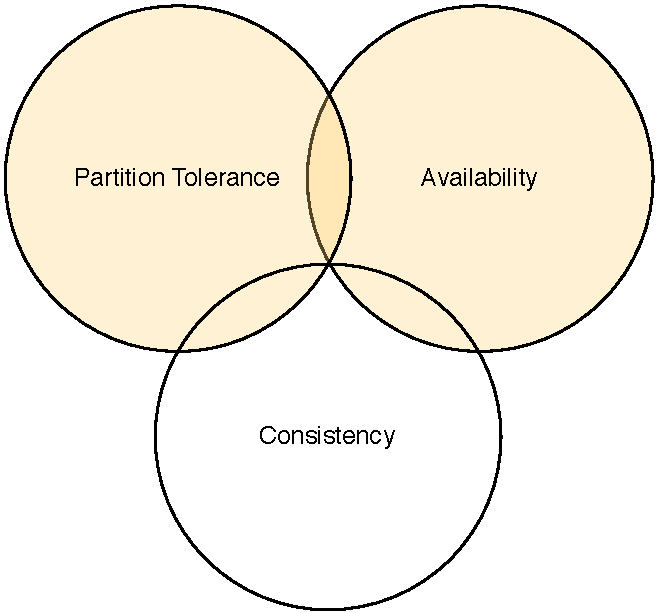
\includegraphics[width=0.5\textwidth]{images/cap}
  \end{center}
  \caption{CAP Theorem}
  \label{fig:cap}
\end{figure}

Consistency essentially means that a read always return the most recently written value, which is guaranteed to happen when the state of a write is consistent among all nodes that have that data (the updates have a global order). Most NoSQL implementations, including Cassandra, focus on availability and partition tolerance, relaxing the consistency guarantee, providing eventual consistency.  

Eventual consistency is seen by many as impracticable for sensitive data, data that cannot be lost. The reality is not so black and white, and the binary opposition between consistent and not-consistent is not truly reflected in practice, there are instead degrees of consistency such as serializability and causal consistency\todo{get reference}. In the particular case of Cassandra the consistency can be considered tuneable in the sense that the number of replicas that will block on an update can be configured on an operation basis by setting the consistency level combined with the replication factor (Section \ref{sec:consistency}).


\section{Data Model}
\label{sec:cass_data_model}
Usually, NoSQL implementations are key-value stores that have nearly no structure in their data model apart from what can be perceived as an associative array. On the other hand, Cassandra is a row oriented\footnote{It is frequently referred to as column oriented, and this is not wrong in the sense that it is not relational. But data in Cassandra is actually stored in rows indexed by a unique key, but each row does not need to have the same columns (number or type) as the ones in the same column family.} database system, with a rather complex data model\cite{sarkissian09}, that is described below.

The basic building block of Cassandra are columns (Fig. \ref{fig:column}) that consist of a tuple with three elements, a name, a value and a timestamp. The name of column can be a string but, unlike its relational counterpart, can also be long integers, UUIDs or any kind of byte array.

\begin{figure}[htb]
  \begin{center}
    \leavevmode
    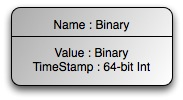
\includegraphics[width=0.3\textwidth]{images/column.jpg}
  \end{center}
  \caption{Cassandra Column}
  \label{fig:column}
\end{figure}

Sets of columns are organized in rows that are referenced by a unique key, the row key, as demonstrated in figure \ref{fig:row}. A row can have any number of columns that are relevant, there is no schema binding it to a predefined structure. Rows have a very important feature, that is that every operation under a single row key is atomic per replica, despite the number of columns affected. This is the only concurrency control mechanism provided by Cassandra.

\begin{figure}[!htb]
  \begin{center}
    \leavevmode
    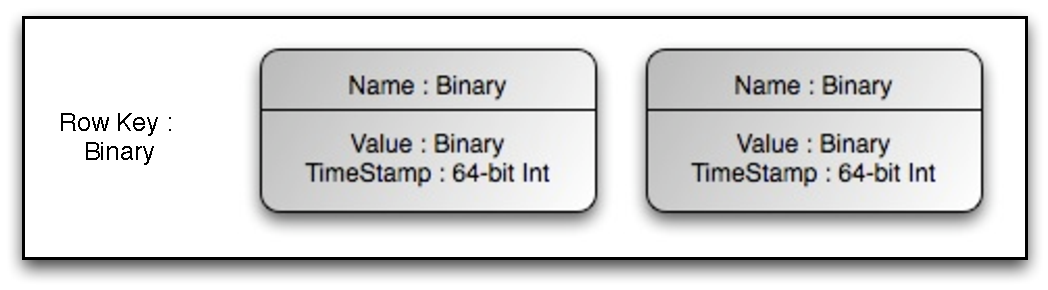
\includegraphics[width=0.8\textwidth]{images/row}
  \end{center}
  \caption{Cassandra Row}
  \label{fig:row}
\end{figure}

The maximum level of complexity is achieved with the column families, which ``glue'' this whole system together, it is a structure that can keep an infinite\footnote{Limited by physical storage space} number of rows, has a name and a map of keys to rows as shown in picture \ref{fig:columnfamily}. 

Applications can specify the sort order of columns within a column family, based on their name, and order them by its value in bytes, converted to an integer or a string, or even as a 16-byte timestamp.

\begin{figure}[!htb]
  \begin{center}
    \leavevmode
    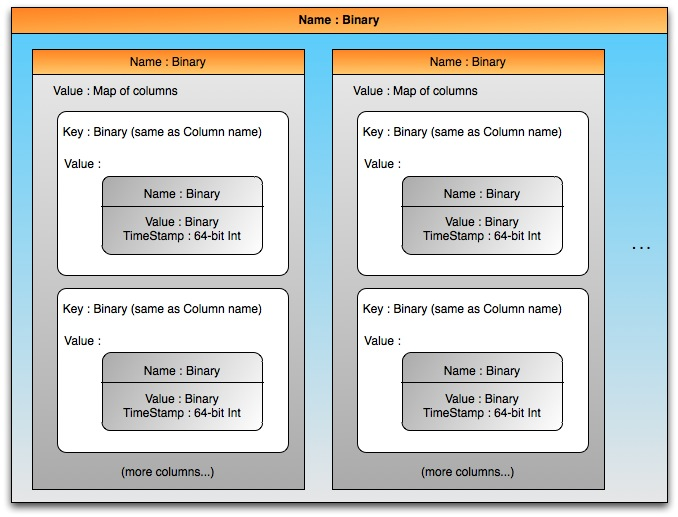
\includegraphics[width=0.8\textwidth]{images/columnfamily}
  \end{center}
  \caption{Cassandra ColumnFamily}
  \label{fig:columnfamily}
\end{figure}


Cassandra also provides another dimension to columns, the SuperColumns (Fig. \ref{fig:supercolumn}), these are also tuples, but only have two elements, the name and the value. The value has the particularity of being a map of keys to columns (the key has to be the same as the column's name).

\begin{figure}[htb]
  \begin{center}
    \leavevmode
    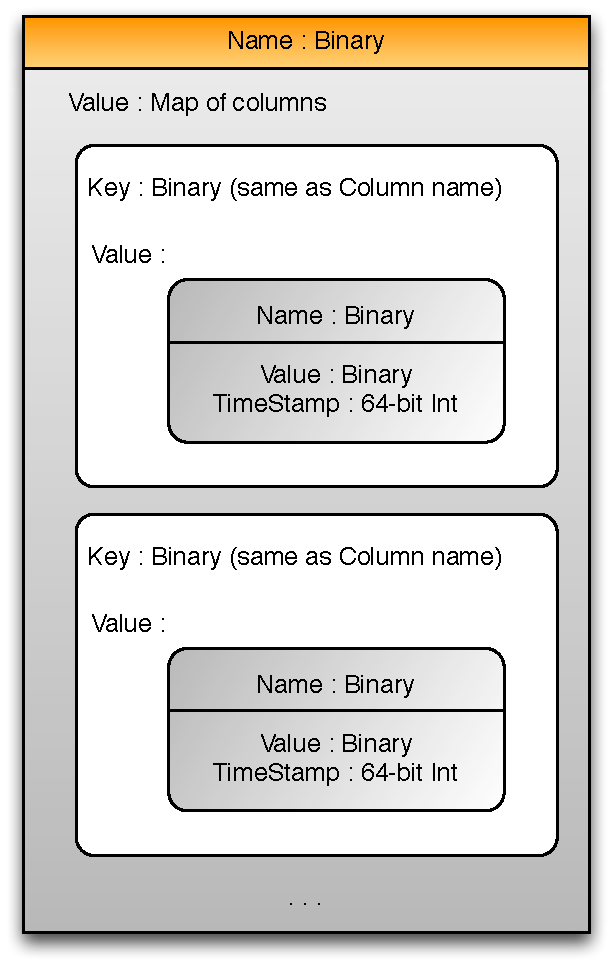
\includegraphics[width=0.4\textwidth]{images/supercolumn}
  \end{center}
  \caption{Cassandra SuperColumn}
  \label{fig:supercolumn}
\end{figure}

There is a variation of ColumnFamilies that are SuperColumnFamilies. The only difference is that where a ColumnFamily has a collection of name/value pairs, a SuperColumnFamily has subcolumns (named groups of columns). This is better understood by looking at the path a query takes until reaching the desired value in both a normal and super column family (Table \ref{tab:path}).

\begin{table}[h!]
\centering
  \begin{tabular}{ l | l }
	\hline \hline
	\textbf{Normal} & Row key $\rightarrow$ Column name $\rightarrow$ Value\\
    \textbf{Super}  & Row key $\rightarrow$ Column name $\rightarrow$ Subcolumn name $\rightarrow$ Value\\
    \hline \hline
  \end{tabular}

\caption{Path to get to value}
\label{tab:path}
\end{table}

Multiple column families can coexist in an outer container called keyspace. The system allows for multiple keyspaces, but most of deployments have only one.

\subsection{Partitioners}
\label{sec:partitioners}

Partitioners define the way rows are ordered in Cassandra. By default the one used is the Random partitioner that combines MD5 hashes of the keys with consistent hashing\footnote{``Consistent hashing is a scheme that provides hash table functionality in a way that the addition or removal of one slot does not significantly change the mapping of keys to slots. By using consistent hashing, only K/n keys need to be remapped on average, where K is the number of keys, and n is the number of slots.'' in Wikipedia, 13/12/2010}) to determine the place where these keys belong in the ring (Section \ref{sec:consistency}). This spreads the keys evenly trough the ring due to its random distribution, but also makes it very inefficient\footnote{most of the times a range query would imply returning the whole set of keys, and filter it.} to perform (even impossible to do from the Cassandra client). 

Since our work relies largely on performing range queries on keys composed of byte arrays, the partitioner used is the Byte-Ordered Partitioner. It is an Order-Perserving Partioner\footnote{Rows are stored by key order, aligning the physical structure of the data with that order} that treats the data as raw bytes, instead of converting it to strings.    


\section{Querying}
Cassandra's \ac{api} defines its querying capabilities, and consists of three simple methods\footnote{The actual client API has more methods that are variations of these or schema related} \cite{lakshmanMalik}:

\begin{itemize}
	\item \emph{update(table, key, rowMutation)}
	\item \emph{get(table, key, columnName)}
	\item \emph{delete(table, key, columnName)}
\end{itemize}	

In the method signatures above, \emph{columnName} can refer to a specific column in a column family, a column family, normal or super, or a column in a supercolumn. The \emph{rowMutation} specifies the changes to the row in case it was already there, or the row to be added\footnote{Cassandra treats inserts as updates to inexistent rows, that is the reason there is no insert operation}, Mutations can also be Deletions that represent deletes when performing a batch update.

\section{Consistency}
\label{sec:consistency}
Cassandra allows clients to specify the desired consistency level on reads and writes, based on the replication factor previously defined in a configuration file, present in every cluster. Notice that if R + W > Replication Factor, where R is the number of nodes to block for on read, and W the ones to block for on write, the most consistent behavior will be achieved\footnote{Because the replication process only requires a write to reach a single node to propagate, a write which ``fails'' to meet consistency requirements will still appear eventually as long as it was written to at least one node.}. Obviously his affects the performance and availability, since all update operations must wait for the update to occur in every node.\\

Cassandra uses replication to achieve high availability and durability. Each data item is replicated at N nodes, where N is the afore mentioned replication factor, assigning each key to a coordinator node (chosen through consistent hashing, that in addition to storing locally each key within his range, replicates these keys at the N-1 nodes in the consistent hashing ring. 

Cassandra system elects a leader amongst its nodes using Zookeeper \cite{Junqueira2007}, that is contacted by all joining nodes, and tells them for what ranges they are responsible. The leader also makes an effort for maintaining the invariant that no node is responsible for more than N-1 ranges in the ring. 

In Cassandra every node is aware of every other node in the system and, therefore the range they are responsible for.


\section{Cassandra as a data store for Derby}

The integration of Cassandra with Derby meant doing two things, defining the way data will be stored and translating Derby operations to Cassandra's API. 

\subsection{Adopted data model}
\label{sec:data_model}
The way the data is organized in Cassandra is a very important feature of this work and influences the design of the integration with Derby. This was, therefore, a feature that had to be carefully thought from the ground up. The various design decisions and the reasons supporting them will be thoroughly explored in the following paragraphs.

This model is not application specific and as such is optimized to the extent it can go without losing its generality. Having this in mind, our design uses one keyspace per relational table, named ``TableXXXX'' with XXXX being the table's conglomerate id\footnote{Derby calls tables and indexes conglomerates, and each of them has a unique id, in our case we use the table id to uniquely identify a keyspace}, with each of these keyspaces having two column families, one for the actual records (\emph{BaseColumns\_CF}) and one for the unique and secondary indexes (\emph{BaseRowLocation\_CF}).

\subsubsection{Indexing in Cassandra}
Secondary indexes where introduced to Cassandra in version 0.7, they allow querying by value and can be built in the background automatically without blocking reads or writes. 

We have not used this, however, because there are still several limitations such as not being recommended for attributes with high cardinality, i.e. attributes that have a lot of unique values, and with these indexes only equality queries can be done, not range queries\cite{secindexlimitations}.

In those cases where these limitations cannot be tolerated (such as ours) the documentation recommends using a separate column family and implement our own secondary index\cite{secindex}. \\ 

The rows in each of the previously mentioned column families have a particular structure. In the case of \emph{BaseColumns\_CF}, the row key is the primary key and the row has one column with name ``valueX'', where X is the position of the relational column, for each value inserted. In the case of \emph{nulls}, that must be inserted in an relational database and therefore are present in the \ac{sql} queries, they are simply ignored, as there is no need to create a column for them since Cassandra has no fixed schema.  

The indexes column family deals with two different situations, when it is a unique secondary index and when it is a non-unique secondary index. In both cases, all columns except one have the name ``keyX'', which follows the same logic as ``valueX'', also the row key is the indexed value or values\footnote{rows with secondary indexes can be indexed on multiple values}. In one hand, when the index is unique, the different column has the name ``location'' with the location of the actual record as a value. On the other hand, when it is a non-unique secondary index, the same column has the location of the record as name and no value (Fig. \ref{fig:mymodel}).

\begin{figure}[htb]
  \begin{center}
    \leavevmode
    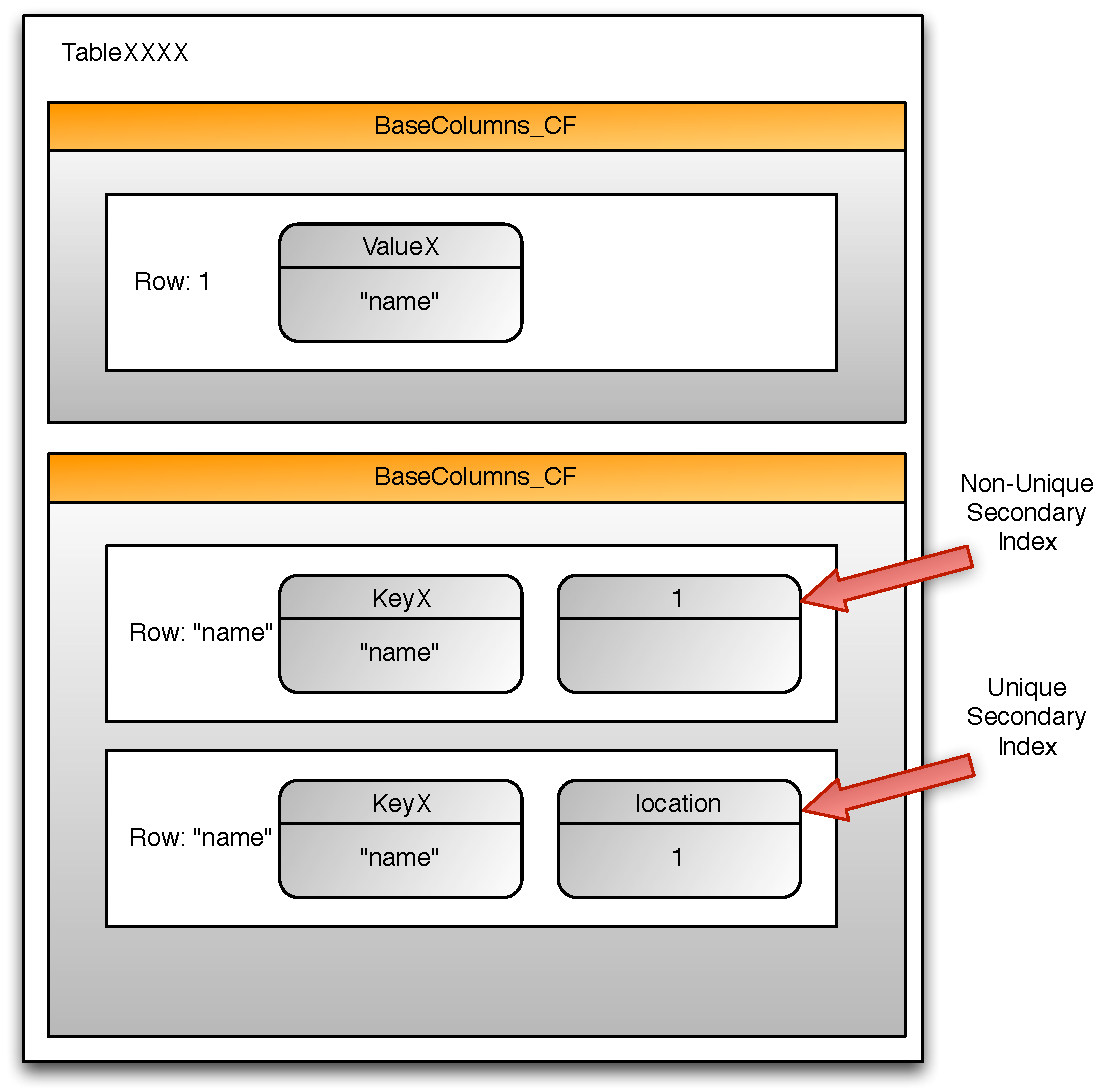
\includegraphics[width=0.7\textwidth]{images/mymodel}
  \end{center}
  \caption{Cassandra design to integrate with Derby}
  \label{fig:mymodel}
\end{figure}

\subsection{Derby operations in Cassandra}
\label{sec:cassandraops}

The various Derby operations that interact with the underlying data store had to be rewritten to be compliant with Cassandra. These operations encompass the creation and deletion of keyspaces, the insertion, replacement, fetching and deletion of rows, as well as the scans or range queries.

\subsubsection{Keyspace operations}
Since version 0.7 of Cassandra it is possible to alter keyspaces definitions on runtime, which allows us to create and delete them\footnote{keyspaces correspond to the relational tables, in our implementation}.

Therefore, when an \ac{sql} create table statement is issued, a keyspace is created, with the name defined according to the model and the replication factor and strategy coming from a configuration file. At the moment of creation of a keyspace, the column family is also created, taking into account if it is an index or not. The deletion is achieved through a call to the provided \emph{system\_drop\_keyspace} method.

While testing the system, we found some problems with this \emph{system} methods that allow the alteration of keyspaces. The main problem is that when a new keyspace is created, the method does not wait for the schema to agree. While this provides better performance since it does not block, it also means that if you try to do a query or an insert on that keyspace before the agreement of the schema, you will get an error that the system cannot come back from. We had to create our own method to wait for the schema agreement to avoid this errors.      

\subsubsection{Row operations}
The operations performed to a row are the insert, replace, fetch and delete and as with the keyspaces they differ from indexes to normal records.

The insertion of a row consists on creating a column for each value, following the data model, and doing a batch update. For this operation the differences between indexes and normal records are not many, and are defined in section \ref{sec:data_model}. 

The replacement of a row only makes sense on normal records, since the indexes are managed internally. There are two main types of row replacements, when the row is complete (the primary key is going to change) and when it is not. If the row is complete and has an index, it is deleted and the new row is inserted (which will update the indexes), if it is not the new columns are added to Mutations and applied in a batch. Since this does not alter the primary it key, there is no need to update the indexes.

When fetching a row the mechanism described in section \ref{sec:derby_scans} takes place in order to increase performance. In those cases where this optimization cannot be applied, what happens is that the necessary values (it is not mandatory to query for the entire row) are fetched and a Derby row is created and passed on.  

Rows are deleted with the API method \emph{remove}, which marks them as deleted for a certain time\footnote{this amount of time is called \emph{GCGraceSeconds} and is defined in cassandra's configuration file}. The reason a row is not deleted immediately is because of the fact that the \emph{remove} is actually performing a distributed delete, which means that some of the replicas may not receive the delete operation. In that case, if the data was to be deleted at once, when one of those replicas becomes available again it will treat the replicas that received the delete as having missed a write update, and repair them. That is why deleted data is replaced with a special Cassandra value called tombstone, that can later be propagated to the replicas that missed the initial remove request.

The reason for this tombstones to be available for a pre defined amount of time is that in a distributed system without a coordinator, it is impossible to know the moment when all the replicas are aware of the delete and it is safe to remove the tombstone. By default Cassandra waits ten days before removing this tombstones.

\subsubsection{Scan operations}
The scanning mechanism starts when the scan controller is initiated, since it is at this time that the range to query is defined and the columns are fetched from the data store. From this point on the controller works with the fetched data in memory.

Both with normal records and indexes the primary method is \emph{fetchNext}, which returns the next row in the range. In the first case, this consists in getting the next row from the iterator and encoding the values to create a Derby row. 

In the second case it is a bit more complex since the indexes can be of three types, which means doing things a little different for each of the types. First, the row is constructed with values that are stored alongside with the location in order to be able to perform the optimization in section \ref{sec:derby_scans} and in the case of primary indexes that is all that is done, except for the validation of the row before it is returned. 

For the other types of indexes the location of the actual record must be fetched as well. In the case of unique indexes the column with name ``location'' is fetched and in the case of non-unique secondary indexes the remaining column has the location as its name. This location is added to the previously constructed row that is then validated and returned.

When performing scans in Cassandra there is one detail to take in account, that are the range ghosts. Cassandra had a range query method that eliminated tombstones from the result set, but has been deprecated due to performance issues. Therefore, when iterating over the rows it is necessary to be aware that a row coming from a range query can have no columns at all, if it has been deleted and is now a tombstone.  

